%version of 08-09-19

\chapter{Graphs II:
Graphs within Computation and Communication}
\label{ch:Graphs2}
\index{graph}

Chapter~\ref{ch:Graphs1} has laid the groundwork for an intensive study of the many 
ways in which graphs and graph-related concepts find application within the fields of 
computing and communicating.  That chapter largely focused on properties of
graphs---and families of graphs---that are local and descriptive: What is the essence of
a graph's being a tree? a hypercube?  The current chapter takes the next step and studies
how the described local structure influences some of the dynamically applicable characteristics
of graphs.  Two major foci in this chapter are {\em vertex-coloring} (Section~\ref{sec:graph-color})
and {\em path discovery} (Section~\ref{sec:path-cycle-problems}).  Both of these topics are used
algorithmically in myriad applications of graphs, from circuit layout to computation scheduling
to interprocessor communication scheduling.  We provide a layered presentation to both topics:
we completely cover the basic aspects of both topics; we offer extended material in appendices,
providing further study opportunities for the interested reader; and we provide pointers to the 
literature for a number of fascinating more-advanced topics.  We close the chapter with capsule
discussions of several specialized topics which go beyond the scope of any introductory text.  We 
hope that the reader will be excited by these preliminary excursions into some occurrences of
graph theory in ``real life".


%{\Denis Introduce here this new chapter. I just checked the content...}

%%%%%%%%%%%%%%%%%%%%%%%%%%%%%

\section{Graph Coloring and Chromatic number}
\label{sec:graph-color}
\index{graph!vertex-coloring}

\index{graph!chromatic number}
This section introduces the notion of {\it graph coloring}, and its
associated notion of the {\it chromatic number} of a graph.

\index{graph!vertex-coloring}
\index{graph!chromatic number} 
A {\it vertex-coloring} of a graph $\g$ is an assignment of labels to $\g$'s vertices, 
in such a way that all of a vertex $v$'s neighbors get a different label than $v$.  Traditionally,
the labels are called {\it colors}, for that term's evocative power.  The {\it chromatic number} of a graph
$\g$ is the smallest number of colors that can be used in a legal
vertex-coloring of $\g$.  In traditional parlance, the assertions

``$\g$ has chromatic number $c$'' \ \ \ \ \ and \ \ \ \ \
``$\g$ is {\it $c$-colorable}''
\index{graph!$c$-colorable}

\noindent
are considered to be synonymous.

\ignore{********
{\Denis I added the following remark, do you agree?}
This notion is an important characteristic of a graph.
It is like an intermediate concept between the degree (local)
and diameter (global), which are both easy to compute. 
Determining the chromatic number is not easy to compute for any graphs.
\bigskip
*********}

\noindent \fbox{
\begin{minipage}{0.95\textwidth}
The notion of graph coloring can be used to computational advantage to
model a broad variety of situations.  An extremely important, and
illustrative, use of graph coloring is to model {\it distributed}
computing.  In this setting, the vertices of a computation-graph $\g$
represent {\it agents}, such as, e.g., processing elements in a
computer; and $g$'s edges represent {\it communication links} that
enable each vertex $u$ to check its neighbors' states before any action
and to inform its neighbors of state-changes occasioned by an action of $u$.  
%{\Denis actually, coloring is useful in any situation to express incompatibility between items}
The prohibition against ``monochrome'' edges---i.e., edges
both of whose incident vertices have the same color---guarantees that
vertex $u$ and all of its like-colored vertices can act at the same instant
with no fear of missing an important input to those actions.  Indeed,
one often encounters programs for distributed computing that look something like

1. All {\em red} vertices perform simultaneously an action

2. All {\em green} vertices perform simultaneously an action

3. All {\em blue} vertices perform simultaneously an action

\hspace*{1in} $\vdots$
\end{minipage}
}

\bigskip

Most of the ``named'' graphs in Section~\ref{sec:graphs-important-families} have 
quite small chromatic numbers.  This is no accident: These graphs were invented (or, at
least, placed in the spotlight) because of their importance to the arena of parallel and
distributed computing---and we suggested in the previous paragraphs how to use graph
vertex-colors to efficiently orchestrate many such computations.  Motivated by this
application of graph models, we devote the current section to studying graphs that
have small chromatic numbers.

\subsection{Graphs with chromatic number $2$}
\label{sec:2-color-graphs}

We begin our study of graphs having small chromatic numbers by focusing on
$2$-colorable graphs, which enjoy the smallest nontrivial chromatic number.
It is not difficult to characterize these graphs structurally.

A graph $\g$ is {\it leveled} \index{graph!leveled} if there exists
an assignment of {\it level numbers} $\{ 1, 2, \ldots, \lambda\}$ to the
vertices of $\g$ in such a way that every neighbor of a level-$\ell$ vertex
$u$ resides either on level $\ell +1$ or on level $\ell -1$.

\begin{prop}
\label{thm:leveled=2-color}
A graph $\g$ has chromatic number $2$ if, and only if, it is leveled.
\end{prop}

\begin{proof}
Say first that $\g$ is a leveled graph.  Then labeling each vertex of
$\g$ with the (odd-even) parity of its level provides a valid
$2$-coloring of $\g$.

Say next that $\g$ is $2$-colorable.  Pick any vertex $v$ of $\g$ and
assign it to be the unique vertex on level $1$.  Let all neighbors of
$v$ be assigned to level $2$.  Continuing iteratively, say that the
largest level-number that we have employed---i.e., assigned vertices
to---is $\ell$.  Then we now assign to level $\ell +1$ all neighbors
of level-$\ell$ vertices which have not yet been assigned to a level of
$\g$.  Because $\g$ is $2$-colorable, each of the levels we have
specified is monochromatic, so that each edge of $\g$ connects a vertex
of one color with a vertex of the other color.  \qed
\end{proof}

We can now show that the following named graphs are $2$-colorable.

\begin{corol}
\label{thm:list-2-colorables}
The following graphs are leveled, hence have chromatic number $2$:

{\bf (a)}
any tree (which includes any path-graph $\p_n$)

{\bf (b)}
any cycle-graph $\cc_n$ that has an even number $n$ of vertices

{\bf (c)}
any mesh-graph $\m_{m,n}$

{\bf (d)}
any torus-graph $\widetilde{\m}_{m,n}$ that has an even number of
diagonals, i.e., even $m+n$

{\bf (e)}
any hypercube $\q_n$
\end{corol}

\begin{proof}
We provide a detailed sketch for each of the five graph families in turn.

\noindent {\bf (a)}
We follow the procedure from the second half of the proof of
Proposition~\ref{thm:leveled=2-color} to expose a level structure in
any tree $\t$, as follows.  Pick any vertex $v$ of $\t$ and make it the
unique vertex on level $1$.  Let all neighbors of $v$ be assigned to
level $2$.  Continuing iteratively, say that the largest level-number
that we have employed is $\ell$.  Then we now assign to level $\ell
+1$ all neighbors of level-$\ell$ vertices which have not yet been
assigned to a level of $\t$.

Of course this process can be simplified when $\t$ is a path-graph
$\p$, by choosing one of $\p$'s end-vertices as vertex $v$.  We thereby
have precisely one vertex on each level, whereas the general procedure
can have levels with $2$ vertices.  A lesson here is that {\em a graph
  may admit many distinct level structures}.

\medskip

\noindent {\bf (b)}
When we apply the procedure of part (a) to an even-length cycle
$\cc_{2q}$, we produce a level structure in which levels $1$ and $q+1$
have one vertex apiece, while all other levels have two vertices apiece.

\medskip

\noindent {\bf (c)}
The edge-structure of mesh-graphs ensures that the labeling of each
vertex $\langle i,j \rangle$ of $\m_{m,n}$ with the odd-even parity of
the number $i+j$ is a $2$-coloring of $\m_{m,n}$.

\medskip

\noindent {\bf (d)}
The labeling in part (d) provides a $2$-coloring of any torus-graph
$\widetilde{\m}_{m,n}$ with even $m+n$.

\medskip

\noindent {\bf (e)}
Each edge of a hypercube $\q_n$ connects a vertex $v = \beta_1 \beta_2
\cdots \beta_n$, where each $\beta_i \in \{0,1\}$, to a vertex $v' =
\beta'_1 \beta'_2 \cdots \beta'_n$ where precisely one $\beta_j$
differs from $\beta'_j$.  Therefore, the following aggregation of
vertices of $\q_n$ into sets $S_0, S_1, \ldots, S_n$ provides a valid
leveling of $\q_n$.

\smallskip

Assign vertex $v = \beta_1 \beta_2 \cdots \beta_n$ to set $S_k$
precisely if $k$ of the bits $\beta_i$ equal $1$.

\medskip

\noindent
The preceding explanations complete the proof.
\qed
\end{proof}

A simple argument verifies that no odd-length cycle $\cc_{2q+1}$ with
$q \geq 1$ is $2$-colorable.  One can craft such an argument by trying to $2$-color
such a cycle.  One can then extend this argument to prove that no graph $\g$
that {\em contains} an odd-length cycle can be $2$-colored.
Containing odd-length cycles is the feature that prevents $2$-colorings of many graphs, 
including the torus $\widetilde{\m}_{m,n}$ when $m+n$ is odd and all de Bruijn networks.

Let us focus momentarily on de Bruijn networks, because they have quite interesting
cyclic sub-digraphs.  One observes the directed $3$-cycle
\[ 00 \ \rightarrow \ 01 \ \rightarrow \ 10  \rightarrow \ 00 \]
in $\d_2$ in Fig.~\ref{fig:dB2by2} and the $3$-cycle
\[ 001 \ \rightarrow \ 010 \ \rightarrow \ 100 \ \rightarrow \ 001 \]
in $\d_3$ in Fig.~\ref{fig:dB2by3}.  In fact, these small odd-length cycles are only the
proverbial tip of the proverbial iceberg for de Bruijn networks.  The following result
asserts that de Bruijn networks are {\it directed-pancyclic}, meaning that 
{\em they contain (even directed!)~cycles of {\em all} possible lengths, both odd and even}.
The proof of this result is outside the scope of an introductory text, but the treatment
in \cite{Yoeli62} should be accessible to the motivated reader.
\index{graph!pancyclic} 
\index{de Bruijn network!pancyclicity}
\index{de Bruijn graph!pancyclicity}


\begin{prop}{\cite{Yoeli62}}
For all $n$, the order-$n$ de Bruijn network $\d_n$ is directed-pancylic, i.e., it
contains directed cycles of all possible lengths $1, 2, \ldots, 2^n$.
\end{prop}

\subsection{Planar and Outerplanar Graphs}
\label{sec:planar+outerplanar-color}
\index{planar graphs}
\index{outerplanar graphs}
\index{graph!planar}
\index{graph!outerplanar}

In this section, we focus on two graph families that are defined in
terms of the way they can be drawn (on a two-dimensional medium, such
as a piece of paper).
\bigskip

\noindent \fbox{
\begin{minipage}{0.95\textwidth}
The reader should not view this attention to how a graph can be drawn
as just an abstract game.  The process of designing and implementing
circuits within the constraints of {\it VLSI}, {\it Very Large Scale Integrated Circuit}
technology, are very similar to drawing a circuit on a two-dimensional medium. 
\index{VLSI} 
\index{Very Large Scale Integrated Circuit technology}
\index{VLSI:Very Large Scale Integrated Circuit technology} 
We refer the reader to the revolutionary 1979 text \cite{Mead-Conway} for an introduction 
to this fascinating technology, which requires technical literacy but little specialized knowledge.
\end{minipage}
}
\bigskip

\index{planar graphs}
\index{graph!planar}
\index{graph!outerplanar}
\index{outerplanar graphs}
\noindent
A graph is {\it planar} \index{graph!planar} precisely if it can be drawn {\em without any crossing edges}.
A graph $\g$ is {\it outerplanar} precisely if it can drawn by {\em placing its vertices along a circle
in such a way that its edges can be drawn as noncrossing chords of the circle}.  The latter condition is
equivalent to demanding that $\g$'s edges can be drawn within the circle without any crossings.

We urge the reader to garner intuition about the graphs in these
families by experimenting with drawing some specific, rather complex graphs.
\begin{itemize}
\item
The first set of graphs to draw are cliques, as defined in
Section~\ref{sec:clique}.  The cliques $\k_3$, $\k_4$, and
$\k_5$ will help expose the nature of the planar and outerplanar
graphs, because:
  \begin{itemize}
  \item
$\k_3$ is outerplanar; 
  \item
$\k_4$ is planar but not outerplanar;
  \item
$\k_5$ is not planar.
  \end{itemize}

\item
The {\em bipartite} cousins of the cliques will also yield valuable insights.  For positive 
integers $m$ and $n$, the $m \times n$ bipartite clique $\k_{m,n}$ is the graph
whose vertex-set comprises the ordered pairs of integers:\index{bipartite clique}
\[  \n_{\fk_{m,n}} \ = \
\{ \langle i,j \rangle \ \ | \ \ 1 \leq i \leq m; \ \ 1 \leq j \leq n\}
\]
and whose edges connect each vertex $\langle i,j \rangle$ to every vertex
$\langle i,k \rangle$ with $1 \leq k \leq n$ and to every vertex
$\langle h,j \rangle$ with $1 \leq h \leq m$.

The second set of graphs to draw are the bipartite cliques $\k_{1,3}$,
$\k_{2,3}$, and $\k_{3,3}$.  These graphs will also help expose the
nature of the planar and outerplanar graphs, because:
  \begin{itemize}
  \item
$\k_{1,3}$ is outerplanar; 
  \item
$\k_{2,3}$ is planar but not outerplanar;
  \item
$\k_{3,3}$ is not planar.
  \end{itemize}
\end{itemize}

We selected the preceding cliques and bipartite cliques to ``play with'' very carefully.
Using arguments that go beyond the scope of this text, one can prove the following
{\em characterization via exclusion} result, which characterizes each of our graph families by
identifying {\it forbidden subgraphs}.  \index{forbidden subgraphs}
\index{forbidden subgraphs!characterization of planar graphs}
\index{forbidden subgraphs!characterization of outerplanar graphs}
The notion of {\it graph homeomorphism} plays a fundamental role in the characterization.
\index{graph!homeomorphism}\index{graph!homeomorph}
This is a dauntingly named technical term that is easily understood informally.
A {\it homeomorph} of a graph $\g$ is obtained by adding (degree-$2$) vertices along one
or more edges of $\g$.  The characterization of planar graphs by exclusion resides in a
celebrated theorem by the Polish mathematician and logician Kazimierz Kuratowski; the
analogous result for outerplanar graphs was derived by the French mathematician Gary
Chartrand and the American mathematician Frank Harary (who invented the name ``outerplanar", as
we describe in Section~\ref{sec:planar-graphs}).
\index{Kuratowski, Kazimierz}
\index{Chartrand, Gary}
\index{Harary, Frank}
 
\begin{theorem}
\label{thm:planar+outerplanar-exclusion}
{\bf (a)} {\rm \cite{ChartrandB67}}
A graph is outerplanar if, and only if, it does not have a subgraph
that is homeomorphic to either $\k_4$ or $\k_{2,3}$.

{\bf (b)} {\rm \cite{Kuratowski30}}
A graph is planar if, and only if, it does not have a subgraph
that is homeomorphic to either $\k_5$ or $\k_{3,3}$.
\end{theorem}


\subsubsection{Outerplanar graphs}

We look first at the smaller of this section's graph families, namely,
the {\it outerplanar graphs}. \index{outerplanar graphs}
We begin our discussion with some basic facts about this family.

\begin{prop}
Every tree is outerplanar.
\end{prop}

We leave the challenge of proving this property to the reader.   As an aid, we provide in
Fig.~\ref{fig:treeoutplanar} an outerplanar drawing of the tree $\t$ Fig.~\ref{fig:tree}.
Specifically, the figure illustrates how one can distribute the vertices of $\t$ around a circle 
in a way that allows one to draw $\t$'s edges in a noncrossing manner.
\begin{figure}[hbt]
\begin{center}
       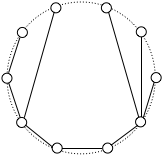
\includegraphics[scale=0.5]{FiguresGraph/TreeOutplanar}
       \caption{Outerplanar representation of the tree of Fig.~\ref{fig:tree}.}
  \label{fig:treeoutplanar}
\end{center}
\end{figure}

\begin{prop}
\label{thm:basic-outerplanar-stuff}
Let $\g$ be an outerplanar graph.  Then:

\begin{tabular}{ll}
{\bf (a)} &
$\g$ is planar. \\
\ignore{********
{\bf (b)} & $\g$ is a subgraph of a Hamiltonian graph. 
{\Denis I removed the second item since Hamiltonian has been shifted after this section.}\\
*********}
{\bf (b)} &
Every subgraph of $\g$ is outerplanar. \\
{\bf (c)} &
At least one of $\g$'s vertices has degree $\leq 2$.
\end{tabular}
\end{prop}

\begin{proof}
{\bf (a)}
$\g$'s planarity can be inferred from our ability to draw $\g$'s edges as noncrossing 
chords of the circle.

\medskip
\ignore{*********
\noindent {\bf (b)} $\g$'s ``sub-Hamiltonianicity'' can be inferred
from the ability to draw $\g$ with its vertices along a circle.

\medskip
*************}

\noindent {\bf (b)} 
We can produce a drawing of any subgraph  $\g'$ of $\g$ that witnesses $\g'$'s outerplanarity 
by erasing some vertices and/or some edges from our outerplanarity-witnessing drawing
of $\g$.  These erasures cannot introduce any edge-crossings.

\medskip

\noindent {\bf (c)}
One verifies easily that part (c) holds for all outerplanar graphs having $3$ or fewer vertices.
Focus, therefore, on an arbitrary outerplanar graph $\g$ that has more than $3$ vertices.  Since
adding more edges to a graph cannot decrease the degree of any vertex, we lose no generality
by focusing on a graph $\g$ that is {\em maximally} outerplanar,  in the sense that adding any
new edge to $\g$ would destroy our ability to draw $\g$'s edges in a noncrossing manner.
\index{maximal outerplanar graph}

Because $\g$ has more than $3$ vertices, and because all of its vertices lie on a circle
(in the drawing that witnesses $\g$'s outerplanarity), there must be pairs of vertices of 
$\g$ that are not adjacent along the circle.  Let $u$ and $v$ be nonadjacent vertices such 
that the distance between $u$ and $v$ (measured in term of number of edges that must 
be traversed to reach one vertex from the other) is minimal among pairs of nonadjacent 
vertices.  We must consider two cases.
\begin{itemize}
\item
If the distance between $u$ and $v$ were {\em exactly} $2$, then the unique vertex
that lies between $u$ and $v$ along the circle would have degree $2$.
\item
If the distance between $u$ and $v$ {\em exceeded} $2$, then there would be at least
{\em two} vertices that lie between $u$ and $v$ in either direction around the circle.
But in this case, there would be two nonadjacent vertices that were closer to one another
than $u$ and $v$---which contradicts our choice of $u$ and $v$ as a pair of {\em closest}
nonadjacent vertices.
\end{itemize}
We conclude that $\g$ must have a vertex of degree $\leq 2$.  \qed
\end{proof}

\bigskip

Our primary concern in this section is, of course, on graph coloring.
We return to this topic now.  The $3$-vertex cycle $\cc_3$ witnesses the
fact that not every outerplanar graph is $2$-colorable; $3$ colors is
the best that we can hope for.  We now show that this hope can be
realized.  The inductive proof of the following result can easily be
turned into an efficient vertex-coloring algorithm for outerplanar
graphs.

\begin{prop}[The $3$-Color Theorem for Outerplanar Graphs]
\label{thm:OP-3-colorability}
Every outerplanar graph is $3$-colorable.
\end{prop}

\begin{proof}
We proceed by induction on the number of vertices in the outerplanar
graph to be colored.

The base cases of the result are provided by small outerplanar
graphs---say those having $3$ vertices or fewer.

We assume, for induction, that every outerplanar graph having fewer
than $n$ vertices is $3$-colorable.

Focus on an arbitrary $n$-vertex outerplanar graph $\g$.  By
Proposition~\ref{thm:basic-outerplanar-stuff}(d), $\g$ has a vertex $v$
of degree $\leq 2$.  Let us remove vertex $v$ from $\g$, along with the
edge(s) that connect $v$ to the rest of $\g$; call the resulting graph
$\g'$.  Now: 
\begin{itemize}
\item
$\g'$ is clearly outerplanar, once we ``stitch'' together the circle that we ``damaged'' 
by removing $v$;
\item
$\g'$ has fewer than $n$ vertices.
\end{itemize}
By induction, therefore, $\g$ is $3$-colorable.  But now we can reattach vertex $v$ to $\g'$
by replacing the edges that attach $v$ to $\g$.  Moreover, we can now color $v$ using
whichever of the $3$ colors on $\g$ that is {\em not} used for $v$'s neighbors in $\g$.
We have, thus, specified a $3$-coloring of $\g$, which extends the
induction and completes the proof.  \qed
\end{proof}

\ignore{**************
Two remarks about Proposition~\ref{thm:OP-3-colorability}:
\begin{enumerate}
\item
Our proof of the proposition can easily be transformed into an
algorithm that $3$ colors any $n$-vertex outerplanar graph in a
number of inductive stages that is a low-degree polynomial in $n$.
\item
The color-bound of the proposition can, of course, not be improved, as
witnessed by odd-length cycle-graphs.
\end{enumerate}
*************}


\subsubsection{Planar graphs}
\label{sec:planar-graphs}

 \index{planar graphs} \index{graph!planar}
The larger of this section's two graph families comprises {\it planar graphs} i.e., graphs
that can be drawn (on a two-dimensional medium, such as a piece of
paper) with no crossing edges.

\bigskip

\noindent \fbox{
\begin{minipage}{0.96\textwidth}
Historically, the original focus on planar graphs stemmed from viewing them as abstractions
of geographical maps:  The political units on a map (countries and/or cities and/or \ldots)
became the vertices of a graph $\g$.  And, units that shared a border were connected by an
edge of $\g$.  The chromatic number of $\g$ was, quite literally, the numbers of shades of
ink that one would need in order to print the map in a way that assigned different colors to
units that shared a border.
\end{minipage}
}

\bigskip

\noindent
In a clique, every pair of vertices are neighbors of each other.  Therefore:

\smallskip

{\em For all $n$, the $n$-vertex clique $\k_n$ can be colored with $n$ colors but no fewer.}

\smallskip

\noindent
As a conseqence, the $4$-vertex clique $\k_4$ witnesses the fact that not every planar graph
is $3$-colorable.

\bigskip

\index{Appel, Kenneth}  \index{Haken, Wolfgang}

\noindent
A century-plus attempt to prove that $4$ colors suffice for planar graphs culminated in one 
of the most fascinating dramas in modern mathematics, as American mathematicians
Kenneth Appel and Wolfgang Haken---with the help of their families and of their
computer!---announced their two-article-long proof in 1974 of their renowned
{\it $4$-Color Theorem for Planar Graphs}.  \index{The $4$-Color Theorem for Planar Graphs}
\index{coloring planar graphs!the $4$-Color Theorem}

\begin{theorem}[The $4$-Color Theorem for Planar Graphs~\cite{AppelH77a,AppelH77b}]
\label{thm:Four-ColorTheorem}
Every planar graph is $4$-colorable.
\end{theorem}

\index{The $4$-Color Problem for planar graphs} 
The proof of Theorem~\ref{thm:Four-ColorTheorem} is beyond the scope
of any introductory text, but the backstory of the proof is truly fascinating---and it 
supplies ample motivation for the proofs of the $6$-color and $5$-color analogues
of the Theorem.  Beginning with a failed attempt in 1875 to prove that every planar
map can be $4$-colored, the so-called {\it $4$-Color Problem} held the world of discrete 
mathematics in thrall for roughly a century before Appel and Haken announced their proof of the Theorem~\ref{thm:Four-ColorTheorem}.  But, this proof notwithstanding,
the drama surrounding the $4$-Color Problem persisted,
because of the Appel-Haken proof's reliance, in a fundamental way, on
a computer program that checked more than a thousand essential---but
clerical---assertions (about forbidden subgraphs).  It took the
mathematics community years before the Appel-Haken proof, with its massive
complexity and unprecedented employment of ``collaboration'' by
computer, was generally accepted.  Even readers who might be daunted by the primary
references \cite{AppelH77a,AppelH77b} that accompany our statement of
the Theorem, may well enjoy the much more accessible articles \cite{AppelH77c,AppelH89}
in which the authors summarize---and, at a rather
sophisticated level, popularize---this marvelous mathematical tale.

\medskip

There are significant lessons within the proofs of the $6$-color and $5$-color
analogues of Theorem~\ref{thm:Four-ColorTheorem}.
\begin{itemize}
\item
The weaker, $6$-color, version of the Theorem can be proved in much the same way as its
outerplanar-graph cousin, Proposition~\ref{thm:OP-3-colorability}.  We now present this proof in detail.  
\item
The proof of the stronger, $5$-color, version of the Theorem already requires us to break the
world into multiple cases---but only a single-digit number of cases, in contrast to the four-digit
case list one encounters with the proof of the Theorem \cite{AppelH77a,AppelH77b}.  That said,
the complexity of the $5$-color theorem has led us to include its proof only in an appendix; see
Chapter~\ref{Appendix:5colors}.
\end{itemize}

\bigskip

\noindent {\it The $6$-Color Theorem for Planar Graphs.}
The first step in showing that every planar graph can be vertex-colored using
$6$ colors resides in the following analogue for planar graphs of
Proposition~\ref{thm:basic-outerplanar-stuff}(d), which asserts that
every outerplanar graph has a vertex of degree $2$.

\begin{lemma}
\label{thm:PlanarGraph-degree5}
Every planar graph has a vertex of degree $\leq 5$.
\end{lemma}

\index{graph!planar!face in a drawing}
\index{planar graph!face in a drawing} 
\begin{proof} {\em (Lemma~\ref{thm:PlanarGraph-degree5})}
Let us focus on a planar drawing of a (perforce) planar graph $\g$
which has $n$ vertices, $e$ edges, and $f$ {\it faces}.  A {\it face}
in a drawing of $\g$ is a polygon whose sides are edges of
$\g$, whose points are vertices of $\g$, and whose interiors are empty,
in that no edge of $\g$ crosses through the interior.

\bigskip

\noindent \fbox{
\begin{minipage}{0.95\textwidth}
Now that we know about faces, we can finally describe the origin of the term {\it outerplanar}.
A graph $\g$ is outerplanar if it can be drawn (on a $2$-dimensional medium) in the following 
manner.  All of $\g$'s vertices are placed around a circle, and all of $\g$'s edges are drawn as 
noncrossing chords of the circle.  The region outside the vertex-bearing circle is, thus, the
{\em outer} face of this special planar drawing of $\g$.
\end{minipage}
}
\bigskip

The following auxiliary result derives a celebrated ``formula'' attributed to Euler.  \index{Euler, Leonhard} \index{Euler's Formula}

\begin{prop} [Euler's Formula for Planar Graphs]
\label{thm:Euler-Formula}
Given the indicated drawing of $\g$, we have
\begin{equation}
\label{eqn:Eulers-formula}
n \ - \ e \ + \ f \ \ = \ \ 2
\end{equation}
\end{prop}

\medskip

We defer proving Proposition~\ref{thm:Euler-Formula} so that we can proceed with our ongoing proof of Lemma~\ref{thm:PlanarGraph-degree5}.  We devote Subsection~\ref{subsec:validationEulerFormula} to 
two quite different proofs of Euler's formula.

\medskip

 \index{graph!planar!maximal}
As we approach the next step of the proof, we simplify the setting by
assuming henceforth that $\g$ is connected and that it is {\em maximal}, in the sense that one cannot
add any new edge to the drawing without crossing an existing edge.  This step only strengthen's the
Lemma's conclusion by apparently making it more difficult to find a small-degree vertex.
{\Denis I don't think the notion of maximality is simple, may be we should add a figure here?}
{\Arny The notion certainly helps ME to think about the proof ... but I am probably not
a typical reader, right?  I think that a figure would be very good here.  Maybe it would suffice to
"challenge" the reader to add one more edge to a planar drawing of $\k_5$ or of $\k_{3,3}$ -- or
of both!!}

With the maximality assumption in place, we now adapt a pedagogical tool from
\cite{Berge73}, in order to make the following counting argument
easier to follow.  We construct a {\em directed bipartite} graph {\bf G} which exposes certain
features of $\g$'s structure.  On one side of {\bf G} are the $f$ faces of $\g$; on the other side
are $\g$'s $e$ edges.  {\bf G} contains an arc from each face of $\g$ to
each edge of $\g$ that forms a ``side'' of the polygonal drawing of the face.  Because $\g$ is
a {\em maximal} planar graph, we have:
\begin{itemize}
\item
Each face of $\g$ is a $3$-cycle, hence involves three vertices.
\item
Each edge of $\g$ touches two faces.
\item
Each edge of $\g$ touches two vertices.
\end{itemize}

Let us now put these facts together, and assume, for contradiction,
that every vertex of $\g$ had degree $\geq 6$.  We would then find that
\[
\left[ f \ \ \leq \ \ \frac{2}{3} e \right] \ \ \ \ \mbox{ and } \ \ \ \
\Big[ e \ \ \geq \ \ 3n \Big]
\]
Incorporating these two bounds into Euler's Formula
(\ref{eqn:Eulers-formula}), we arrive at the following contradiction.
\[ 2 \ \ = \ \ n \ - \ e \  + \ f
\ \ \leq \ \ \frac{1}{3} e \ - \ e \ + \ \frac{2}{3} e \ \ = \ \ 0
\]
This contradiction proves that every planar graph must have a vertex of
degree $\leq 5$.
 \qed-Lemma~\ref{thm:PlanarGraph-degree5}
\end{proof}

\medskip

We finally have the tools to color planar graphs using $6$ colors.
\index{The $6$-Color Theorem for Planar Graphs}
\index{coloring planar graphs!the $6$-Color Theorem}

\begin{prop}[The $6$-Color Theorem for Planar Graphs]
\label{thm:P-6-colorability}
Every planar graph is $6$-colorable.
\end{prop}

\begin{proof}
The $2$-Color Theorem for Outerplanar Graphs (Proposition~\ref{thm:OP-3-colorability}) 
and this result follow via almost-identical inductions on the number of vertices in the graph $\g$
that is being colored.  Both arguments:
\begin{enumerate}
\item
remark that the target number of colors is adequate for small graphs

For outerplanar graphs, ``small'' means ``$3$ or fewer vertices''.  For
planar graphs, it means ``$4$ or fewer vertices''.

\item
remove from $\g$ a vertex $v$ of smallest degree $d_v$, together with
all its incident edges

For outerplanar graphs, we guarantee that $d_v \leq 2$ (Proposition~\ref{thm:basic-outerplanar-stuff}(d)).
For planar graphs, we guarantee that $d_v \leq 5$ (Lemma~\ref{thm:PlanarGraph-degree5}).

\item
inductively color the vertices of the graph left after the removal of $v$ (denoting the smaller
graph by $\g'$).

For outerplanar graphs, we color $\g'$ with $\leq 3$ colors (Proposition~\ref{thm:OP-3-colorability}).
For planar graphs, we use an inductive assumption that $\g'$ can be colored with $\leq 6$ colors. 

\item
reattach $v$ via its $d_v$ edges and then color $v$.

Note that the coloring guarantee in both results---Proposition~\ref{thm:OP-3-colorability}
for outerplanar graphs and the current result for planar graphs---allows us to use $d_v +1$ colors 
to color $\g$.  Because $v$ has degree $d_v$, it can have no more than $d_v$ neighboring 
vertices in $\g'$, so our access to $d_v +1$ colors guarantees that we can successfully color $v$.
\end{enumerate}
The proofs of the $3$-colorability of outerplanar graphs and the
$6$-colorability of planar graphs thus differ only in the value of
$d_v$.  \qed
\end{proof}

\bigskip

\noindent {\it The $5$-Color Theorem for Planar Graphs.}
\index{The $5$-Color Theorem for Planar Graphs}
\index{coloring planar graphs!the $5$-Color Theorem}

\bigskip

\begin{prop}[The $5$-Color Theorem for Planar Graphs \cite{Heawood90}]
\label{thm:5colors}
\label{thm:P-5-colorability}
Every planar \\
graph is $5$-colorable.
\end{prop}

\medskip

The proof, being rather technical, is relegated to the
Appendix, as Chapter~\ref{Appendix:5colors}.

\medskip

\ignore{***********
\noindent \fbox{
\begin{minipage}{0.95\textwidth}
The case analysis in the following proof is a bit more complex than in
most of the results in the text, but a methodical reading should make
the proof quite accessible.  Moreover, {\em roadmap} of the case
analysis is a valuable lesson in how mathematics is really done!  For
instance, the motivated reader will be able to recast the totally
positive proof we present into the form of a proof by contradiction.
The positive version should be more to the taste of a computationally
oriented reader---but both proofs are equally correct.
\end{minipage}
}

The proof again (I mean like for 6 colors) is by recurrence but we add
here a contradiction argument:
Similarly, we focus on a vertex with degree 5 (at some points, we will
have to justify this)
This vertex (call it x) has 5 neighbors
The problem is when they are colored by the 5 colors, otherwise it is
colored by a missing one.
Let now label these 5 vertices from 1 to 5.
Consider the vertices 1 and 3, colored by two different colors and the
sub-graph composed of vertices with colors 1 and 3
If these two vertices are in disjoint connected components, (case 1), it is
easy to color x by reverting the colors 1 and 3 in one component
(see figure)
Thus, the problem is when there exists an alternate path (in term of
colors) between vertex 1 and vertex 3
in this case (case 2), consider vertices 2 and 4, using a similar process
as in case 1, if there are two connected components
we are done (x can be colored by reverting the colors along the path
in one component), otherwise, there is an alternate path
between 2 and 4.
However, since the graph is planar, then, both alternate paths will
intersect, which is impossible
************************}

\ignore{***********
\begin{proof}
For brevity, let us henceforth discuss only {\em valid} colorings,
i.e., colorings of a graph's vertices in which neighboring vertices get
different colors.

\smallskip

\noindent {\em Base of our induction.}
Because the $5$-clique $\k_5$ is obviously $5$-colorable, so also must
be all graphs having $\leq 5$ vertices.  Therefore, we know that any
non-$5$-colorable graph would have $\geq 6$ vertices.

\smallskip

\noindent {\em Inductive hypothesis.}
Assume, for induction, that every planar graph having $\leq n$ vertices
is $5$-colorable.

\smallskip

\noindent {\em Inductive extension.}
If the proposition were false, then there would exist a planar graph
$\g$ having $n+1$ vertices which is not $5$-colorable.  By
Lemma~\ref{thm:PlanarGraph-degree5}, $\g$ would have a vertex $v$ of
degree $\leq 5$.  The remainder of the proof focuses on the graph
$\g$, its minimal-degree vertex $v$, and on $v$'s $(d_v \leq 5)$
neighbors in $\g$.

Now, if there were a coloring of $\g$'s vertices in which $\leq 4$ colors
were used to color $v$'s neighbors, then the following analogue of the
coloring strategy of Proposition~\ref{thm:P-6-colorability} would
produce a $5$-coloring of $\g$.
\begin{enumerate}
\item
Remove vertex $v$ and its incident edges from $\g$, thereby producing
the $n$-vertex planar graph $\g'$.
\item
Produce a $5$-coloring of $\g'$ that uses only $4$ colors for the
vertices that are neighbors of $v$ in $\g$.
\item
($a$) Reattach vertex $v$ and its edges to $\g'$, thereby reconstituting
  $\g$.  ($b$) Color $v$ with whichever of the $5$ available colors is
  not used to color $v$'s neighbors.
\end{enumerate}

In order to proceed in pursuit of a contradiction, we must understand
what structural features of $\g$ make it impossible to use only $4$
colors on $v$'s neighbors when $5$-coloring $\g$.  There are three
important situations to recognize.
\begin{description}
\item[{\sf Case 1}.]
Vertex $v$ has degree $\leq 4$.

\smallskip

By definition, $\leq 4$ colors are used to color $v$'s neighbors in
this case.
\end{description}
Note that, in all remaining cases, vertex $v$ has precisely $5$
neighbors---or else, we would have invoked Case 1 to color $\g$ with
$5$ colors.
\begin{description}
\item[{\sf Case 2}.]
For some $5$-coloring of $\g$, $\geq 2$ neighbors of $v$ get the same
color.

\smallskip

Because $v$ has exactly $5$ neighbors, in this case, only $4$ colors
are used to color these neighbors.
\end{description}
In all remaining cases, the $5$ neighbors of $v$ receive distinct
colors.
\begin{description}
\item[{\sf Case 3}.]
For some $5$-coloring of $\g$, some two neighbors of $v$, call them
$v_1$ and $v_2$, reside in distinct components of $\g$ once $v$ and
its incident edges are removed from $\g$.

\smallskip

As before, let $\g'$ be the (in this case, disconnected) graph that
results when $v$ and its incident edges are removed from $\g$.  For $i
= 1,2$ Let $\g_i$ be the component of $\g'$ that contains vertex $v_i$.

Say that, under the $5$-coloring of $\g$ that we are focusing on,
$v_1$ is colored {\it red} and $v_2$ is colored {\it green}.

Let us recolor the vertices of $\g_1$ so that vertex $v_1$ is now colored
{\it green}.  (One needs only switch the colors {\it red} and {\it
  green} in the existing coloring of $\g_1$.)  It is always possible
to do this in a way that does not affect the valid coloring of $\g_2$
because $\g_1$ and $\g_2$ are mutually disjoint.

Once we have thus-recolored $\g_1$, we have a $5$-coloring of $\g$ for
which Case 2 holds.  (In fact, we can color vertex $v$ {\em red} when we
reattach it to $\g'$.)
\end{description}

\noindent
We now see that Cases 1--3 cannot prevent us from $5$-coloring $\g$, so
we are left with the following minimally constrained situation.
\begin{description}
\item[{\sf Case 4}.]
\begin{itemize}
\item
Every minimum-degree vertex of $\g$ has $5$ neighbors.

For the minimum-degree vertex $v$, let us call these neighbors $v_1$,
$v_2$, $v_3$, $v_4$, $v_5$, in clockwise order within the planar
drawing.
\item
In every $5$-coloring of $\g$, the neighbors of every minimum-degree
vertex receive distinct colors.

For vertex $v$, let us say that neighbor $v_i$ receives color $c_i$.
\end{itemize}
The leftmost graph in FIGURE 1 
{Denis Put right ref here}
depicts the portion of $\g$ comprising
vertex $v$ and its neighbors.  In the figure, we use integer $i$ to
denote, ambiguously, vertex $v_i$ and its assigned color $c_i$.  The
question mark ``?'' that ``colors'' vertex $v$ indicates that we do not
yet know what color to assign to $v$.  The other two graphs in the
figure depict schematically how we have dealt with Case 3 above.
\begin{itemize}
\item
All neighbors of vertex $v$ remain in the same component of $\g$ when
$v$ and its incident edges are removed.
\end{itemize}
\end{description}
To analyze Case 4, we focus on vertices $v_1$ and $v_3$ in FIGURE 1.
{Denis Put right ref here}
Importantly, these vertices have received distinct colors ($c_1$ and $c_3
\neq c_1$, respectively), and these vertices are not adjacent to one
another as one makes a clockwise sweep around vertex $v$.

Now take $\g$ and focus only on the vertices that are colored $c_1$ or
$c_3$ (as are $v_1$ and $v_3$, respectively) and on the vertices that are
colored $c_2$ or $c_4$ (as are $v_2$ and $v_4$, respectively).  One
sees from Figure 2 that:
\begin{itemize}
\item
$\g$ can, {\em but need not}, contain a path whose vertices alternate
  colors $c_1$ and $c_3$---call this a ``$c_1$-$c_3$ path'' between
  vertices $v_1$ and $v_3$.
\item
$\g$ can, {\em but need not}, contain a path whose vertices alternate
  colors $c_2$ and $c_4$---call this a ``$c_2$-$c_4$ path'' between
  vertices $v_2$ and $v_4$.
\item
$\g$ {\em cannot} contain both of the paths just described, i.e., a
  $c_1$-$c_3$ path between $v_1$ and $v_3$ {\em and} a $c_2$-$c_4$ path
  between $v_2$ and $v_4$.

{\em These two paths, if they existed, would cross one another---which
  is forbidden because $\g$ is a {\em planar} graph.}  See Figure 2.
\end{itemize}
It follows that {\em either} $\g$ does not contain a $c_1$-$c_3$ path
between $v_1$ and $v_3$ {\em or} $\g$ does not contain a $c_2$-$c_4$
path between $v_2$ and $v_4$.  Say, with no loss of generality, that
the former path does not exist.  Then we can switch colors $c_1$ and
$c_3$ beginning with vertex $v_1$ and obtain a coloring of $\g$ in which
$v_1$ and $v_3$ both receive the color $c_3$.  We can then proceed as
in Case 2 to get a $5$-coloring of $\g$.

This four-case analysis shows that we can always produce a
$5$-coloring of $\g$, which completes the proof.  \qed
\end{proof}
*****************}

\bigskip

We  close our study of vertex-colorings of planar graphs with an overview of the intellectual
cost-benefit tradeoff that we have exposed:
\begin{itemize}
\item
A straightforward recursive coloring strategy suffices if one is
willing to settle for a $6$-color palette when coloring planar graphs
(Proposition~\ref{thm:P-6-colorability}).
\item
A four-case analysis, in which one case comprises several subcases, is
needed in order to eliminate one of the colors from our palette, i.e., to
achieve a $5$-coloring strategy (Proposition~\ref{thm:5colors}).
\item
An analysis involving close to $2000$ cases is needed in order to
achieve the provable optimal, a $4$-color palette that always works
(Theorem~\ref{thm:Four-ColorTheorem}).
\end{itemize}

\subsubsection{Two validations of Euler's Formula}
\label{subsec:validationEulerFormula}
\index{Euler's Formula}

We develop two quite different proofs of Proposition~\ref{thm:Euler-Formula}.

\medskip

\index{Euler's Formula!validation via structural induction}
\noindent {\bf Validation via structural induction}. 
Our first approach validates (\ref{eqn:Eulers-formula}) by growing a planar graph $\g$
inductively, edge by edge.

\smallskip

\noindent {\it Base case}.
The Formula clearly holds for the smallest planar graphs, including
the smallest interesting one, $\cc_3$, which has $n = e = 3$ and $f =2$
(the inner and outer faces of the ``triangle'').

\smallskip

\noindent {\it Extension}.
We grow the current version of $\g$ by adding a new edge.  Two cases arise.
\begin{itemize}
\item
{\em The new edge connects existing vertices.}
In this case, this augmentation of $\g$ increases the number of edges ($e$) and the
number of faces ($f$) by $1$ each, while keeping the number of vertices
($n$) unchanged.

\item
{\em The new edge adds a new vertex, which is appended to preexisting vertex.}
In this case, this augmentation of $\g$ keeps the number of faces ($f$) unchanged while
it increases by $1$ both the number of edges ($e$) and the number of vertices ($n$). 
\end{itemize}
In both cases Euler's Formula (\ref{eqn:Eulers-formula}) continues to hold as we augment
$\g$.  The augmentation thereby extends the induction, hence validates the Formula.
\qed

\bigskip

%{\Denis Here is a nice alternative proof for the Euler proposition}

\index{Euler's Formula!validation via deconstruction}
\noindent {\bf Validation via deconstruction}.
Let us be given a planar graph $\g$ that has $n$ vertices, $e$ edges, and $f$
faces.  We validate Formula (\ref{eqn:Eulers-formula}) by deconstructing $\g$ and showing
that each step in the process preserves as {\it invariant} the expression
\begin{equation}
\label{eq:phi-in-euler-formula}
 \phi(n,e,f) \ = \ n-e+f
\end{equation}

\bigskip

\index{invariants}
\noindent \fbox{
\begin{minipage}{0.95\textwidth}
\textit{Invariant} are extremely important conceptual tools when crafting proofs.  The underlying idea
is to find an expression $\phi(\cdot)$ whose value is preserved (i.e., ``holds
invariant") as some relevant process proceeds.

Rather than try to explain the concept in abstraction, we recommend that the reader follow this
validation of Euler's Formula while keeping track of the invariance of expression
$\phi(n,e,f)$ of (\ref{eq:phi-in-euler-formula}).
\end{minipage}
}
\bigskip

\noindent
Focus on the following two-phase process.
\begin{description}
\item[{\bf Phase 1}.]
Iterate the process of removing edges from $\g$ until one edge-removal reduces $\g$ to
a graph with a single face.

The reader should verify that this termination condition is  equivalent to stopping when the remaining
graph is a (connected) tree.

{\Arny The proof of termination with a connected tree should be an exercise.}

\bigskip

{\bf The action}.
If the graph remaining at some step contains an edge that is shared by
two distinct faces, then remove any such edge.

\smallskip

Fig.~\ref{fig:planarStep1} illustrates the action of Phase 1 for a
(residual) graph with $n=8$ vertices, $e=11$ edges, and $f=5$ faces.
\begin{figure}[hbt]
\begin{center}
   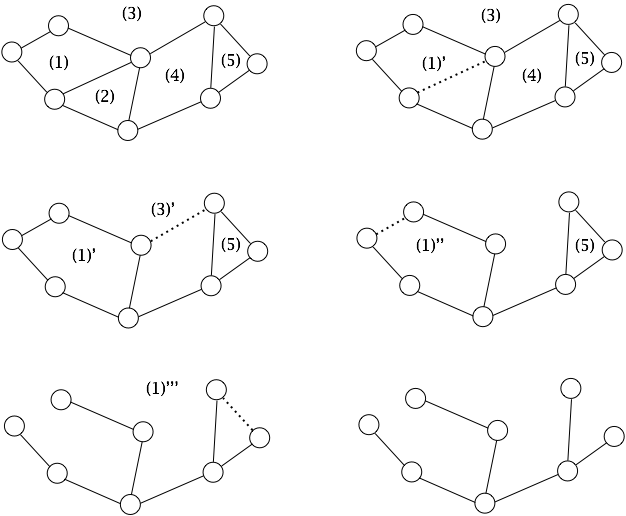
\includegraphics[scale=0.35]{FiguresGraph/planarStep1}
\caption{Illustrating Phase 1: From top left to bottom right, each
  transformation preserves the invariant $\phi(n,e,f)$.  The first
  transformation removes the edge shared by faces (1) and (2),
  creating a new, merged, face (1)'.}
  \label{fig:planarStep1}
\end{center}
\end{figure}

\bigskip

{\bf The analysis}.
\begin{itemize}
\item
The graph remaining after an edge-removal is still planar---because edges are
removed but never added---so we can continue the process.
\item
The process preserves the value of function $\phi$; i.e.,
\[ \phi(n,e,f) \ = \ \phi(n,e-1,f-1) \]
This is because $n$ is unchanged, while $e$ and $f$ are each reduced by $1$.
\end{itemize}

\smallskip

\item[{\bf Phase 2}.]
Iterate the following process of removing vertices from the tree produced
by Phase 1, until only one vertex remains.

\bigskip

{\bf The action}.
Remove any leaf of the current tree, together with its incident edge.

Fig.~\ref{fig:planarStep2} illustrates the action of Phase  2
for a tree  with $n=8$ vertices---hence, $e=7$ edges and $f=1$ face.
\begin{figure}[hbt]
\begin{center}
   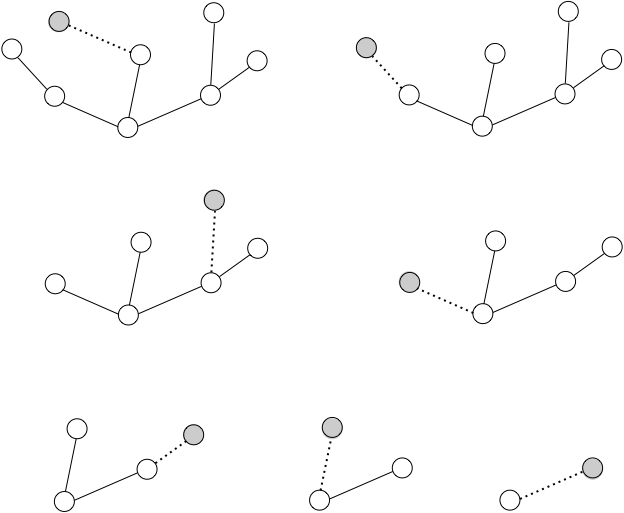
\includegraphics[scale=0.35]{FiguresGraph/planarStep2}
   \caption{Illustrating Phase 2: We remove a sequence of leaves, each
     with its incident edge, until we reach a single vertex.  Here again,
     $\phi$ remains invariant after each leaf-removal.}
  \label{fig:planarStep2}
\end{center}
\end{figure}

\bigskip

{\bf The analysis}.
The value of function $\phi$ remains invariant under each leaf-removal; i.e.,
\[ \phi(n,e,f) \ = \ \phi(n-1,e-1,f) \]
To wit, $f$ is unchanged ($f \equiv 1$ for a tree), while $n$ and $e$ are
each reduced by $1$.
\end{description}

\medskip

\noindent {\bf The cumulative analysis}.
\begin{itemize}
\item
Our process executes a number of steps exactly equal to the number of
edges of the graph $\g$ that we begin with.  Specifically, the edge-removing
Phase 1 removes $e-n$ edges, while the leaf-removing Phase 2 removes $n-1$ vertices.
\item
At the end of the process, $e=0$ and $n=f=1$, so that the residual
value of $\phi$ is $2$.  Because each action prescribed by the process
preserves the value of $\phi$, we know that $\phi$ has the value $2$
before each edge-removal and leaf-removal.
\end{itemize}
We conclude, in summation, that at the start of the process, $\phi(n,e,f)$ had the value $2$.
In other words, $n-e+f = 2$, as asserted by Euler's Formula.   \qed

\bigskip

\noindent \fbox{
\begin{minipage}{0.95\textwidth}
Our study of vertex-coloring in graphs has focused almost entirely on planar and outerplanar graphs.
This is because, aside from the importance of such graphs in applications,  their vertex-coloring
problems can be studied entirely within a mathematical setting (which is our focus).  Vertex-coloring
for broader families of graphs usually proceeds within an algorithmic setting (which is not our focus).
In closing this topic, though, we remark that there are many interesting algorithmic problems relating
to vertex-coloring arbitrary graphs.  The following central such result dates to the earliest days of the 
study of {\sf NP}-completeness.

\smallskip

{\em For any fixed $k \geq 3$, the problem ``Is graph $\g$ $k$-colorable"
is {\sf NP}-complete} \cite{GareyJ79,Karp72}.

\smallskip

The preceding result suggests that {\em optimal} vertex-coloring is computationally difficult.  This
contrasts with the existence of ``greedy'', hence efficient, vertex-coloring algorithms that give quite
good results in practice \cite{CLRS}.  (``Greedy" here refers to algorithms that allocate a yet-unused
color to a vertex only when no uncolored vertex can be validly colored with an already-used color.  
See Footnote~\ref{foot:greedy} in Chapter~\ref{ch:Graphs1}.)
\end{minipage}
}


\section{Path and Cycle Discovery Problems in Graphs}
\label{sec:path-cycle-problems}

Just as various genres of {\it spanning trees} are used to
``summarize'' aspects of the connectivity structure of a 
graph $\g$, various genres of {\it paths} and {\it cycles} in $\g$ are
often useful to ``summarize'' aspects of $\g$'s traversal structure.
This section is devoted to a range of problems related to determining
the existence in a graph $\g$ of a path or a cycle that {\em completely} ``summarizes'' $\g$'s 
traversal structure---either by containing each vertex of $\g$ precisely once or by containing
each edge of $\g$ precisely once.  We generally focus in this section only
on {\em undirected} paths and cycles in {\em undirected}, {\em unweighted} graphs.
Extrapolating the notions we discuss to their directed analogues in directed and/or weighted
graphs, will be accomplished via carefully crafted exercises.  In a similar, but simpler, vein, we 
generally discuss only problems concerning {\em cycles}, leaving to the reader
the analogous path-related notion.  We begin by delimiting the two main
classes of cycle-discovery problems that we study.

\smallskip

\index{graph!Eulerian cycle} \index{Eulerian cycle}
\index{graph!Eulerian circuit} \index{Eulerian circuit} 
\index{Euler, Leonhard}
{\it Eulerian cycles (or, tours)}.  A cycle in a graph $\g$ that traverses each of $\g$'s {\em edges} 
precisely once is called an {\it Eulerian cycle} (or, often, an {\it Eulerian circuit}).  The 
edge-exhausting cycles/circuits/tours referred to by these several names were introduced
as a topic of study in 1736  by the Swiss mathematician Leonhard Euler, whose name we 
have already encountered multiple times.  Euler allegedly identified the topic
while contemplating how to devise a tour of the town of K\"{o}nigsberg
that would cross each of the town's bridges precisely once.  The quest
for Eulerian cycles in graphs is certainly one of the oldest problems---perhaps literally the oldest 
problem---in the fields now called {\it operations research} and {\it graph theory}.  
(An edge-exhausting {\em path} in $\g$ is referred to in the obvious analogous way.)  When one 
views an Eulerian cycle as a ``map'' for traversing a graph---as did Euler when contemplating this
problem---one often calls the cycle an {\it Eulerian tour}. Traditionally, a
graph that admits an Eulerian cycle is said to be {\it Eulerian}. 
 \index{graph!Eulerian tour} \index{Eulerian tour}
 \index{graph!Eulerian} \index{Eulerian graph}

\medskip

\index{graph!Hamiltonian cycle} \index{Hamiltonian cycle}
\index{graph!Hamiltonian circuit} \index{Hamiltonian circuit}
\index{Hamilton, William Rowan} \index{Kirkman, Thomas Pennington}
Dually: A cycle in a graph $\g$ that encounters each of $\g$'s {\em vertices}
precisely once is called a {\it Hamiltonian cycle}, (or, often, a {\it Hamiltonian circuit}).  
This cycle-discovery problem is named in honor of the British mathematician 
Sir William Rowan Hamilton, who is credited with inventing the
concept in the mid-19th century.  (In fact, Hamilton's work on his eponymous cycles
was anticipated by many decades in the work of fellow British mathematician 
Thomas Pennington Kirkman.)  When one views a Hamiltonian cycle as a ``map'' for 
traversing a graph, one often calls the cycle a {\it Hamiltonian tour}.  Traditionally, a graph
that admits a Hamiltonian cycle is said to be {\it Hamiltonian}.  (A vertex-exhausting {\em path} 
in a graph is referred to in the obvious analogous way.)  
 \index{graph!Hamiltonian tour}\index{Hamiltonian tour}
 \index{graph!Hamiltonian} \index{Hamiltonian graph}

\medskip

Despite the conceptual duality between the edge-exhausting goal that underlies Eulerian 
paths and cycles and the vertex-exhausting goal that underlies Hamiltonian paths and cycles,
these two graph-traversing goals differ from one another in virtually every significant
mathematical and algorithmic respect.  It is rather easy to characterize the family of graphs that
admit Eulerian tours and to find such a tour if it exists (Section~\ref{sec:EulerianCycle}); in 
contrast, there is no known characterization of the family of graphs that admit Hamiltonian tours,
and the computational problem of efficiently determining whether a graph admits such a tour is 
one of the major classical problems in the
field of computational complexity  (Section~\ref{sec:Hamiltonian-cycle}).

%%%%%%%%%%%%%%%%%%%%%%%%%%%%%%%%%%%%%%%%%%%%%%%%%%%%

\subsection{Eulerian Cycles and Paths}
\label{sec:EulerianCycle}

The main results in this section characterize the families of directed and undirected graphs
that admit {\it Eulerian cycles} or {\it Eulerian paths}.  The proofs of these characterizations are
constructive: they consist of algorithms that efficiently find such a cycle or such a path when 
one exists.  We focus on graphs that are connected: the algorithms we present can actually be 
adapted to find an Eulerian cycle or an Eulerian path in each connected component of a general graph.

As we embark on our adventure, we note the following amusing fact: \\
{\em The problem of finding an Eulerian cycle in a graph $\g$ is
equivalent to the problem of drawing $\g$ without ever lifting one's
pencil.} \index{graph!drawing without lifting pencil}

\medskip

In the next two propositions, we develop---for both cycles and paths, in both undirected and directed
graphs---simple, elegant characterizations of graphs that admit Eulerian cycles and paths.
These characterization are validated via simple and efficient algorithms that determine
whether a given graph admits such a path or such a cycle.

\begin{prop}[Eulerian Cycles]
\label{thm:eulerian-cycle}
{\bf (a)}
A connected undirected graph $\g$ admits an Eulerian cycle if, and only if,
every vertex of $\g$ has even degree.

{\bf (b)}
A connected directed graph $\g$ admits a directed Eulerian cycle if, and only if,
$\mbox{\sc indegree}(v) \ = \ \mbox{\sc outdegree}(v)$
for every vertex $v$ of $\g$.
\end{prop}

{\Denis The question of edge multiplicity should be addressed somewhere since in particular
the chinese postman is based on edge duplicates...}
{\Arny I do not understand what you are proposing.  If multiple edges occur just in one special
environment, then M. Occam tells us to introduce that complication JUST in that environment,
using the simpler more general situation in the body of the text.  We should discuss}

\begin{proof}
The {\em necessity} of the conditions asserted in parts {\bf (a)} and {\bf (b)} follows from
the following observations.  

{\Arny The original conditions were wrong.  An unconnected
graph CAN have an Eulerian cycle of the type we define, since we do not demand that 
the cycle contains all vertices.  Thus, by our definition, an Eulerian graph remains Eulerian 
if we add isolated vertices to it.  We must discuss this -- should we demand that the cycle
touches all vertices??}


\begin{itemize}
\item
A graph that has no isolated vertices does not admit an Eulerian cycle.
\item
Each Eulerian cycle that a graph admits accounts for two edges per vertex,
because the cycle must ``enter'' the vertex by one edge and ``exit'' by a different edge.
\end{itemize}

\smallskip

\noindent
We turn now to the verification of the {\em sufficiency} of the
Proposition's conditions.  Our argument resides in the following
``streamlined'' version of an induction---this is closer to the form
of an induction that one would encounter in practice, rather than in a
textbook.

The base case of the induction resides in proving the sufficiency of
the Proposition's conditions for ``small'' graphs.  
\bigskip

\noindent \fbox{
\begin{minipage}{0.95\textwidth}
While we largely
leave this step to the reader, we do want to discuss the definition of
``small''.  Until we understand how to deal with arbitrary $n$-vertex
graphs, we will not know how the general step of our induction reduces
the graph size $n$ at each step.  Because of this, it is a good
practice to ``play'' with several small graph sizes initially.
Hopefully, in addition to giving our inductive argument a robust base
case, such ``playing'' will give us valuable intuition for the general
case of the induction.
\end{minipage}
}


\begin{itemize}
\item
Focusing on {\em undirected} graphs: We note that $2$-vertex graphs
cannot have even vertex-degrees---and, indeed, as promised by the
Proposition, they cannot be Eulerian.  One can exhaustively enumerate
all $3$-vertex and $4$-vertex graphs and verify that the Proposition correctly
separates the ones that are Eulerian from those that are not.
\item
Focusing on {\em directed} graphs: We note that $2$-vertex digraphs can be
Eulerian---as witnessed by the $2$-vertex digraph each of whose vertices
hosts a single arc that points to the other vertex.  Once again, one can
perform an exhaustive enumeration of $3$-vertex and $4$-vertex digraphs
and verify that the Proposition correctly separates the Eulerian ones
from the non-Eulerian ones.
\end{itemize}

We now develop a complete proof of the {\em sufficiency} of the
conditions in part {\bf (a)} of the Proposition for general $n$-vertex
undirected graphs.  Throughout the discussion, we intersperse hints
regarding the sufficiency of the conditions in part {\bf (b)} of the Proposition.

Let us consider a connected $n$-vertex undirected graph $\g$ all of
whose vertices have nonzero even degree.
%{\Denis  should'nt multi-vertex be defined? What do you mean here?}

{\Arny Please draft your proposed proof, and we can compare the two approaches.  It is
really hard to discuss this piece by piece.}

{\Arny Also, yesterday I inserted details for a proof similar to this in order to show that a tree has
a vertex of degree $1$ --- See Lemma~\ref{lem:vtx-deg-connected}.  Please look at that proof and 
at this proof to see whether we should craft  a single more general (abstract?) argument 
that works for both.}

\begin{description}
\item[{\bf Step 1}]
Initialize the {\it progress parameter} $k$ to $0$.  This parameter
will help orchestrate our discovery of the Eulerian cycle within $\g$.
{\Denis no need to step 1}

\item[{\bf Step 2}]
Choose an arbitrary vertex of $\g$ some of whose incident edges have not
yet been traversed.  Call this vertex $v_k$, and let us henceforth refer
to $v_k$ as a {\em special} vertex.  Follow a walk along edges of $\g$
beginning at special vertex $v_k$.  
{\Denis we should change $v_k$ to $v$ if we change the way to write the proof...}
The rules of this walk are:
\begin{itemize}
\item
Every step of the walk will traverse an edge of $\g$ that {\em has not yet been traversed} during any walk.
\item
The walk terminates when it encounters a vertex of $\g$ {\em all of
  whose edges have already been traversed}.
\end{itemize}
The facts that 

\hspace*{.25in}\begin{tabular}{ll}
(1) & each vertex of $\g$ has even degree; \\
(2) & the walk begins at vertex $v_k$ (which crosses one of $v_k$'s edges); \\
(3) & no edge of $\g$ is traversed more than once
\end{tabular}

\noindent
mean that the last vertex encountered in this walk is $v_k$.  In other
words: {\em This walk begins and ends with vertex $v_k$.}

{\Arny
\noindent \fbox{
Proposition~\ref{thm:cycle-in-graph} proves that every graph with all degrees $\geq 2$
contains a cycle.}

\noindent \fbox{
Uses pigeonhole to show that  ``leave by a different edge" strategy runs out of new edges.
}
}


Note that vertex $v_k$ will occur in this walk multiple
times---specifically with multiplicity $\frac{1}{2} \mbox{\sc
  degree}(v_k)$.
  
{\Denis I would suggest here to simply a bit, in fact both  steps 1 and 2 aims simply at determining a non-empty cycle in the graph...}

We have completed the walk in $\g$ that begins and ends at vertex $v_k$.

{\Denis I suggest to skip step 3... I think it is enough -- and more easy-- to build
the whole eulerian cycle from any cycle. Do I miss something?}

\ignore{\smallskip
\item[{\bf Step 3}]
Say that we have completed the walk in $\g$ that begins at vertex $v_k$.

{\bf If} every edge of $\g$ has been traversed by the end of the
current walk, then we {\it go to {\bf Step 4}} and invoke procedure
{\bf Build Eulerian Cycle}, which stitches our series of walks into an
Eulerian cycle in $\g$.

\smallskip

{\bf Else}, there is a vertex of $\g$, call it $v_{k+1}$, one of whose
incident edges has not yet been traversed.  Note that we are here
increasing the value of our progress parameter from $k$ to $k+1$.  We
now {\it repeat {\bf Step 2}} with the updated progress parameter,
$k+1$.
}

\item[{\bf Step 4}]
\ignore{We have reached this step because our sequence of walks that begin and
end at special vertices has terminated with all of $\g$'s edges having
been traversed.}

The previous step determined a cycle in graph $\g$,.
Once it is removed, it remains several connected components,
denoted by $\mathcal{C}_1$, $\mathcal{C}_2$, $\ldots$ $\mathcal{C}_c$.
This cycle intersects the strong components at vertices $v_1$, $v_2$ until $v_c$. 
We are now ready to exhibit an Eulerian cycle in $\g$ by going piece after piece along the cycle 
starting from $v_k$.
{\Denis change it to $v$}

\end{description}

\ignore{The resulting procedure
{\bf Build Eulerian Cycle} proceeds as follows.

For each special vertex $v_k$, during the walk that begins and ends at
$v_k$, we encounter other special vertices, call them $v_{k,1}$,
$v_{k,2}$, \ldots, $v_{k,{m_k}}$, in the order of their being
encountered along the walk.  We then define the following recursive
procedure.
{\Denis it is not really recursive since each procedure is only called once...}

\medskip

\begin{tabular}{|ll|}
\multicolumn{2}{l}{{\bf Procedure Build Eulerian Cycle}($v_k$)} \\
\hline
{\bf Phase $1$} &
Follow the walk that begins at $v_k$ until it encounters $v_{k,1}$ \\
  &
Execute {\bf Build Eulerian Cycle}($v_{k,1}$) \\
\hline
{\bf Phase $2$} &
Continue the walk that begins at $v_k$ until it encounters $v_{k,2}$ \\
  &
Execute {\bf Build Eulerian Cycle}($v_{k,2}$) \\
\hline
  &
$\begin{array}{c}
\bullet \\
\bullet \\
\bullet
\end{array}
$ \\
\hline
{\bf Phase $m_k$} &
Continue the walk that begins at $v_k$ until it encounters $v_{k,m_k}$ \\
   &
Execute {\bf Build Eulerian Cycle}($v_{k,m_k}$) \\
\hline
{\bf Phase $m_k +1$} &
Complete the walk that begins at $v_k$. \\
\hline
\end{tabular}
\end{description}

\medskip

\noindent
The process invocation

Execute {\bf Build Eulerian Cycle}($v_0$)

\noindent
produces the Eulerian cycle in $\g$.
}

\bigskip

When dealing with a {\em directed} graph, we proceed exactly as
with undirected graphs, with one critical difference: for each vertex
$v$ we always enter $v$ along one of its {\em in-arcs}, and
we always exit $v$ along one of its {\em out-arcs}.  As in the
undirected case, each arc is traversed precisely once during
the described process.

{\Denis my proof of the proposition is by induction on the number of edges, not vertices...}  \qed
\end{proof}


\ignore{**************
We offer two proofs of this result: the first merely establishes the
existence of the cycle; the second actually computes the cycle.  Both
proofs invoke the following elementary facts.
\bigskip
\noindent {\bf Claim 1.}
if all the degrees are even (and not null) then there exists a cycle.\bigskip
\noindent {\bf Claim 2.}
A tour is an union of disjoint cycles.\bigskip
\noindent {\bf Claim 3.}
If we remove a cycle in a tour then the degrees remain even.\bigskip
\begin{proof}
{\bf A proof of existence.}


The necessary condition of the proposition is straightforward. 
Let us focus on the sufficient condition.
\bigskip

\noindent {\bf Proof 1 (existence).}

By contradiction, let us assume that all the vertices of a connected graph are even and there is no tour that contains all the edges.
Let consider a tour with a maximum number of edges. 
If we remove its edges, it remains some edges and from Claim~3 they are even.
Then, from Claim~1, there exists a cycle within these remaining edges (say $\Gamma$). 
The contradiction comes from Claim~2 since the union of the maximal tour plus the cycle $\Gamma$ 
is another tour which contains more edges than the initial one.
\bigskip

\noindent This proof can be adapted in a constructive way and thus, leads to an algorithm. It is as follows:

\noindent {\bf Proof 2 (constructive).}
By induction on the number of edges. 

\begin{itemize}
\item The basis case is simple to verify for $m=2$ (where two vertices linked by two edges correspond to the cycle of minimal length). 
\item
Let consider a connected graph with $m+1$ edges where all its vertices have an even degree.
Let assume that the property holds for connected graphs of even vertices with $k$ edges ($k \leq m$), which means there exist Eulerian tours in these sub-graphs. 

From Claim~1, there exists a cycle (let denote it by $\Gamma$ described by its successive vertices) and consider the sub-graph of $G$ 
without the edges of $\Gamma$: $G'=(V-{\Gamma},E')$. 
By induction hypothesis, there exists an Eulerian cycle $\mathcal{C}_i$ in each connected component of $G'$ 
(from Claim 3).
The Eulerian tour of $G$ is obtained by the concatenation of pieces of $\Gamma$ and the Eulerian cycles in the successive $\mathcal{C}_i$.

\end{itemize}
*****************}

The simplicity of the preceding characterization degrades a trifle when
one seeks Eulerian {\em paths} rather than {\em cycles}.

\begin{prop}[Eulerian Paths]
\label{thm:eulerian-path}
{\bf (a)}
A connected undirected graph $\g$ admits an Eulerian path if, and only if,
at most two vertices of $\g$ have odd degree.

{\bf (b)}
A connected directed graph $\g$ admits an Eulerian path if, and only if: either $\g$ admits an 
Eulerian cycle, or $\g$ contains one vertex $u$ such that

\hspace*{.5in}$\mbox{\sc indegree}(u) \ = \ \mbox{\sc outdegree}(u) +1$

\noindent
and one vertex $v$ such that

\hspace*{.5in}$\mbox{\sc indegree}(v) \ = \ \mbox{\sc outdegree}(v) -1$.
\end{prop}

The proof of the path-oriented Proposition~\ref{thm:eulerian-path} shares its overall structure
with the proof of the cycle-oriented Proposition~\ref{thm:eulerian-cycle}, with one major difference.
Whereas a cycle has neither beginning nor end, a path has both. 
Proposition~\ref{thm:eulerian-path}(a) asserts that an undirected graph which admits an
Eulerian path but not an Eulerian cycle has precisely two vertices of odd degree, and these 
odd-degree vertices play the roles of the endpoints of the Eulerian path.  In similar fashion,
Proposition~\ref{thm:eulerian-path}(b) asserts that a directed graph which admits an Eulerian
path but not an Eulerian cycle contains one vertex, $u$, whose out-degree exceeds its
in-degree and one vertex, $v$, whose in-degree exceeds its out-degree: vertex $u$ plays the role of
the beginning vertex of the Eulerian path, and vertex $v$ plays the role of the end vertex of the path.
With these hints, we invite the reader to adapt the proof of Proposition~\ref{thm:eulerian-cycle} to
obtain a proof of Proposition~\ref{thm:eulerian-path}.

\bigskip

We close this section by applying Proposition~\ref{thm:eulerian-cycle}
to the ``named graphs" of Section~\ref{sec:graphs-important-families}.

\medskip

{\small
\begin{tabular}{|l|l|l|}
\hline
Graph & Eulerian? & Explanation \\
\hline \hline
Cycle                          & Yes                          & Every vertex has degree $2$ \\
\hline
Clique                         & Odd index only       & $\k_{2n}$ has odd vertex-degrees \\
\hline
2-Dim.~Mesh  & No                           & Non-corner top and side edges have degree $3$ \\  
\hline                     
2-Dim.~Torus  & Yes                          & Every vertex has degree $4$ \\
\hline
Hypercube                  & Even index only & Every vertex of $\q_n$ has degree $n$ \\
\hline
de Bruijn                     & Yes  & Directed: Vertices have equal {\sc indegree} and {\sc outdegree} \\
                                   &         & Undirected $\d_n$: vertices $\overline{0}$ and $\overline{1}$ have
                                                  degree $2n-2$ each; \\
                                    &.       & \hspace*{.77in}all other vertices have degree $2n$ \\
\hline
\end{tabular}
}
\ignore{******************
{\Denis May be we should briefly summarize what happens for these graphs 
(hypercubes with even orders, etc.)}
\medskip

The significance of the de Bruijn network in both coding and
computation (as discussed in Section~\ref{sec:deBruijn}) lends
considerable weight to the following important application of
Proposition~\ref{thm:eulerian-cycle}:  When combined with
Proposition~\ref{thm:deBruin-linegraph-EX}, we obtain a proof of 
Proposition~\ref{thm:deBruijn-Hamiltonian}.

\begin{corol}
\label{thm:deBruijn-Eulerian}
Every de Bruijn network $\d_n$ is (directed)-Eulerian.
\end{corol}
********************}

%%%%%%%%%%%%%%%%%%%%%%%%%%%%%%%%%%%%%%%%%

\subsection{Hamiltonian Paths and Cycles/Tours}
\label{sec:Hamiltonian-cycle}

We turn now to the problem of determining when a connected graph $\g$
has a {\it Hamiltonian cycle}---and the allied problem of finding such
a cycle when one exists.  One can envision a number of benefits
rendered accessible by the presence of a Hamiltonian cycle in a graph
$\g$.  Most obviously, the cycle specifies a tour of $\g$ (or of a map
whose structure $\g$ abstracts) which visits each of $\g$'s vertices
precisely once.  This is the sense in which the cycle ``summarizes"
$\g$'s traversal structure.

\subsubsection{More inclusive notions of Hamiltonianicity}

Many graphs---even ones with ``nice'' structures---do not admit
Hamiltonian cycles.  The reader can generate {\it mesh-graphs}
(Section~\ref{sec:mesh}) that admit no Hamiltonian cycle.  The
existence of such non-Hamiltonian graphs has spawned several
independent paths of inquiry.  One path seeks ``modest'' ways to
weaken the property of {\it Hamiltonianicity}
\index{graph!Hamiltonianicity} in a way that retains many of
Hamiltonianicity's benefits while encompassing a broader range of
graph structures.  We describe two avenues toward weakened, more
inclusive, notions of Hamiltonianicity.

\noindent {\it Be satisfied with paths, rather than cycles}.
A {\it Hamiltonian path} \index{graph!Hamiltonian path}
\index{Hamiltonian path} in a graph $\g$ is a path that passes through
each of $\g$'s vertices precisely once.  Hamiltonian paths can easily be
shown to be a strictly weaker notion than Hamiltonian cycles, in the
obvious sense where every graph that admits a Hamiltonian
cycle also admits a Hamiltonian path: one just drops any single edge
of such a cycle to obtain such a path.  However, there are many graphs
that admit a Hamiltonian path that do not admit any Hamiltonian cycle.
As suggested earlier, there exist mesh-graphs that admit no
Hamiltonian cycle, even though every mesh-graph admits a Hamiltonian
path.  This latter claim is verified by a path that traverses the rows
of a mesh-graph {\it seriatim}, in alternating directions.

\noindent {\it Be satisfied with short paths, rather than edges}.
A Hamiltonian cycle in graph $\g$ is a circular enumeration of $\g$'s
vertices in which adjacent vertices are at unit distance from one
another---i.e., are connected by an edge.  We can weaken (or,
generalize) this notion to create a {\it Hamiltonian $k$-cycle}
\index{graph!Hamiltonian $k$-cycle} in $\g$, for any positive integer
$k$: This is a circular enumeration of $\g$'s vertices in which adjacent
vertices are at distance $\leq k$ from one another---so a Hamiltonian
$1$-cycle is what we have been calling a Hamiltonian cycle.  In fact,
the following result shows that one need not let $k$ be very big
before one encompasses all connected graphs.  Regrettably, the proof
of this result is beyond the current text.

\begin{prop}
\label{thm:weak-Hamiltonianicity}
{\bf (a)} {\rm \cite{ChartrandK69}}
Let $\g$ be any connected graph.  One can cyclically enumerate the
vertices of $\g$ in such a way that vertices that are adjacent in the cycle
are at distance $\leq 3$ in $\g$.


\noindent {\bf (b)} {\rm  \cite{Fleischner74}}
Let $\g$ be any graph that is {\em $2$-connected}
\index{graph!$2$-connected} \index{graph!biconnected} (or, {\it
  biconnected}) in the sense that, for every two vertices, $u$ and $v$,
of $\g$, there exist at least two vertex-disjoint paths in $\g$ that
connect $u$ and $v$.  One can cyclically enumerate the vertices of $\g$
in such a way that vertices that are adjacent in the cycle are at
distance $\leq 2$ in $\g$.
\end{prop}

\subsubsection{Hamiltonianicity in ``named'' graphs}
\label{sec:hamilonian-named-graphs}

Yet another direction of inquiry is to determine whether specific
graphs of interest are Hamiltonian.  We illustrate this avenue by
reviewing the five important families of graphs we studied in
Section~\ref{sec:graphs-important-families}.

\begin{prop}
\label{thm:named-graph-Hamiltonian}
{\bf (a)}
Every cycle-graph $\cc_n$ is Hamiltonian.

\noindent {\bf (b)}
Every clique-graph $\k_n$ is Hamiltonian.

\noindent {\bf (c)}.1.
For all $m,n$: the mesh-graph $\m_{m,n}$:

(i)  is path-Hamiltonian.

(ii) contains no odd-length cycle; hence, is not Hamiltonian if $mn$
is odd.

(iii) is Hamiltonian whenever $mn$ is even 

\noindent {\bf (c)}.2.
For all $m,n$: the torus-graph $\widetilde{\m}_{m,n}$ is Hamiltonian.

\noindent {\bf (d)}
Every hypercube $\q_n$  is Hamiltonian.

\noindent {\bf (e)}
Every de Bruijn network $\d_n$ is (directed)-Hamiltonian.
\end{prop}

\begin{proof}
\noindent {\bf (a)}
This is a tautology, by definition of $\cc_n$.

\medskip

\noindent {\bf (b)}
This is immediate because, by definition, $\k_n$ contains every
$n$-vertex graph---including $\cc_n$---as a subgraph.

\medskip

\noindent {\bf (c)}.1.i.
As we noted earlier in the text, one can ``snake'' a path through
$\m_{m,n}$, row by row, from the top-most to the bottom-most.  By
``snake'', we mean that one should traverse adjacent rows in
alternating directions.

\noindent {\bf (c)}.1.ii.
This is a consequence of the fact that $\m_{m,n}$ is {\it bipartite}:
\index{graph!bipartite} One can color $\m_{m,n}$'s vertices red and blue
in such a way that every edge connect vertices of different colors.
Details are left to the reader.

\noindent {\bf (c)}.1.iii.
We sketch the construction of a Hamiltonian cycle in $\m_{m,n}$ when
$mn$ is even.  Say, with no loss of generality that $m$ is even, so
that $\m_{m,n}$ has an even number of rows.  Temporarily remove column
$1$ of $\m_{m,n}$, and consruct the ``snaking'' Hamiltonian path
described in part {\bf (c)}.1.i of this proof.  Because $m$ is even,
this path begins and ends in column $2$ of $\m_{m,n}$.  One can,
therefore, replace column $1$ and use it to connect the ends of the
``snaking'' Hamiltonian path.  This describes a Hamiltonian cycle in
$\m_{m,n}$.

\noindent {\bf (c)}.2.
When $mn$ is even, the Hamiltonianicity of $\widetilde{\m}_{m,n}$
follows from the fact that $\m_{m,n}$ is a spanning subgraph of
$\widetilde{\m}_{m,n}$.  (Think about it!)  When $mn$ is odd, one
needs just traverse $\widetilde{\m}_{m,n}$'s vertices row by row, going
to the cyclically next vertex after completing each row (see Fig.~\ref{fig:HamiltonTorus}).  
Details of the formal proof are left to the reader.
\begin{figure}[hbt]
\begin{center}
       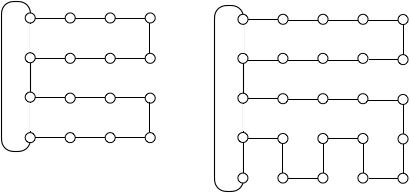
\includegraphics[scale=0.6]{FiguresGraph/HamiltonTorus}
       \caption{Principle for building hamiltonian cycles in torus (even-even and odd-odd).}
  \label{fig:HamiltonTorus}
\end{center}
\end{figure}
\medskip

\noindent {\bf (d)}
One can craft a Hamiltonian cycle in $\q_n$ by
generating an {\it order-$n$ binary reflected Gray code}---so named
for its inventor, Bell Laboratories researcher \index{Gray, Frank}
Frank Gray; see \cite{PetersonW81}.  \index{Gray code} \index{binary
  reflected Gray code} Such a ``code'' is a cyclic enumeration of all
$2^n$ binary strings of length $n$ having the property that cyclically
adjacent \index{strings!cyclically adjacent} strings differ in only
one bit-position.  Length-$n$ strings $x_i$ and $x_j$ are {\it
  cyclically adjacent} in the Gray code $\langle x_0, \ x_1, \ldots,
x_{2^n-1} \rangle$ if $j = i+1 \bmod 2^n$.

\noindent
It is computationally easy to generate an order-$n$ Gray code from an
order-$(n-1)$ Gray code, as follows.

We note first that the order-$1$ code is the sequence $\langle 0, 1
\rangle$.

Inductively, to generate the order-$(k+1)$ Gray code from the
order-$k$ code:
\begin{itemize}
\item
Concatenate the order-$k$ code with a {\em reversed} copy of itself.
(It is the code-sequence that is reversed, not the individual strings.
For instance, as we go from the order-$2$ code $\langle x_0, \ x_1,
\ x_2, \ x_3 \rangle$ to the order-$3$ code, we concatenate that
sequence with $\langle x_3, \ x_2, \ x_1, \ x_0 \rangle$.)
\item
Augment each length-$k$ string in one copy of the order-$k$ Gray code
to length $(k+1)$ by prepending a $0$ to each string; and, augment
each length-$k$ string in the other (reversed) copy of the order-$k$
Gray code to length $(k+1)$ by prepending a $1$ to each string.
\end{itemize}
The following table illustrates the first few steps of this process.
\begin{equation}
\label{eq:gray-code}
 {\small
\begin{array}{|c|c|c|c|}
\hline
\mbox{Order } \ 1
  & \mbox{Order } \ 2
  & \mbox{Order } \ 3
  & \mbox{Order } \ 4 \\
\hline
0   & 00   & 000  &  0000 \\ 
1   & 01   & 001  &  0001 \\
    & 11   & 011  &  0011 \\
    & 10   & 010  &  0010 \\
    &      & 110  &  0110 \\
    &      & 111  &  0111 \\
    &      & 101  &  0101 \\
    &      & 100  &  0100 \\
    &      &      &  1100 \\  
    &      &      &  1101 \\  
    &      &      &  1111 \\  
    &      &      &  1110 \\  
    &      &      &  1010 \\  
    &      &      &  1011 \\  
    &      &      &  1001 \\  
    &      &      &  1000 \\  
\hline
\end{array} }
\end{equation}

We now sketch a proof that for each index $n \in \N^+$, the order-$n$ Gray code sequence
specifies a Hamiltonian cycle in $\q_n$; exercises will give the reader the opportunity to fill 
in details.  We verify the following two assertions in turn:
\begin{enumerate}
\item
{\it The order-$n$ Gray code contains all $2^n$ length-$n$ binary strings.}
\item
{\it Every pair of cyclically adjacent strings in the order-$n$ Gray code differ in a single bit-position.}
\end{enumerate}
{\it Verification}.

\noindent {\it Assertion} 1.
We sketch the induction.  When $n=1$, the Gray code consists of
the two distinct strings $0$ and $1$.  Assume that the assertion holds
for $n=k$.  The order-$(k+1)$ code is obtained by taking two copies of
the order-$k$ code and prepending $0$ to the strings in one copy and
$1$ to the strings in the other copy.  The $2^k$ distinct binary
strings from the order-$k$ code thereby produce $2^{k+1}$ distinct
binary strings in the order-$(k+1)$ code.

\medskip

\noindent {\it Assertion} 2.
We distinguish three situations.  Let the adjacent strings be string $x$, which appears in 
position $i$ of the code, and string $y$, which appears in position $i+1 \bmod 2^n$ of the code.
  \begin{itemize}
  \item
Say that $i = 2^n-1$.  In this case $x$ is the last string in the
code, and $y$ is the first string.  By the ``reflective'' nature of the
construction of the code, we know that $x = 1z$ and $y = 0z$ for some
length-$(n-1)$ binary string $z$.  Strings $x$ and $y$ therefore
differ in precisely one bit-position, namely, bit-position $0$.

  \item
Precisely the same argument shows that when $i = 2^{n-1} -1$, strings
$x$ and $y$ again differ precisely in bit-position $0$.

  \item
In all other cases, namely, when $i \in \{0,1, \ldots, 2^n-1\}
\setminus \{2^{n-1} -1, 2^n-1\}$, strings $x$ and $y$ share the same
first bit-position.  In fact, for some bit $\beta \in \{0,1\}$, $x =
\beta u$ and $y = \beta v$ for length-$(n-1)$ binary strings $u$ and
$v$ which are cyclically adjacent in the order-$(n-1)$ Gray code.  By
an inductive argument, $u$ and $v$ differ in precisely one
bit-position---which means that $x$ and $y$ also differ in precisely
one bit-position.
  \end{itemize}
  The previous analysis is summarized in Fig.~\ref{fig:HamiltonHypercude} for $n=4$.
  \begin{figure}[hbt]
\begin{center}
       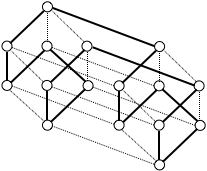
\includegraphics[scale=0.6]{FiguresGraph/HamiltonHypercube}
       \caption{Hamiltonian cycle (bold) in Hypercube using reflected Gray codes.}
  \label{fig:HamiltonHypercude}
\end{center}
\end{figure}


\noindent {\bf (e)}
By Proposition~\ref{thm:deBruin-linegraph}, each de Bruijn network $\d_n$ is the 
line-digraph of the next bigger de Bruijn network, $\d_{n+1}$.  Therefore, by definition
of ``line (di)graph'', the fact that $\d_n$ is (directed)-Eulerian (Corollary~\ref{thm:deBruijn-Eulerian})
means that $\d_{n+1}$ is (directed)-Hamiltonian.  \qed
\end{proof}


\subsubsection{Testing general graphs for Hamiltonianicity}
\label{sec:Hamiltonian-unweighted}

The techniques we use in Section~\ref{sec:hamilonian-named-graphs} to investigate 
the Hamiltonianicity of our ``named'' graphs exploit the detailed structures of the individual 
graphs.  Thus, we cannot expect the proof of Proposition~\ref{thm:named-graph-Hamiltonian} 
to suggest avenues for determining whether an arbitrary given graph is Hamiltonian.  In
fact, quite sophisticated results proved in the early 1970s make a strong mathematical
argument that no set of case studies is likely to have a major impact on the problem of 
testing general graphs for Hamiltonianicity.  This is because, in common with the Satisfibility
problem {\sf 3SAT} of Section~\ref{sec:Satisfiability}, the Hamiltonianicity-detection problem is 
{\sf NP}-complete.  We repeat from our discussion in Section~\ref{sec:Satisfiability} that the
details of the theory of {\sf NP}-completeness are beyond the scope of
this text, but we do want the reader to recognize the following.
\begin{description}
\item
{\it The problem of deciding, given a graph $\g$ that is presented via a list of vertices and a 
list of edges, whether $\g$ admits a Hamiltonian path or a Hamiltonian cycle is {\sf NP}-complete.}
\end{description}


%%%%%%%%%%%%%%%%%%%%%%%%%%%%%%%%%%%

\section{$\oplus$ Pointers to Advanced Topics}
\label{sec:advanced-topics}

%**PROVIDE SOME REFERENCES

We conclude this chapter by mentioning a variety of topics that are
typically not covered---at least in depth---early in the curriculum,
but that are important enough that the reader should at least be aware
of them.  The topics we mention are motivated by virtually every
computational area that benefits from graph-theoretic models.  We have
tried to present each topic at a level of discourse that
will prepare the interested reader to delve more deeply into the
material, yet at a level of informality that will make the material
accessible to the more casual reader.  We thus strive for an intuitive
presentation that will not lead any reader astray.

The problem that we discuss in Section~\ref{sec:Relate-CS-Math-Probs}
illustrates how the {\em dynamic} models in the field of
algorithmics---``dynamic'' in the sense that they {\em do}
something---and the {\em structural} models provided by graph theory
can often provide beneficial illumination of one another.

\index{graph!graph separators}\index{graph!graph decomposition}
Section~\ref{sec:graph-decompose} focuses on the myriad computations
on graphs that can be accomplished efficiently via recursive algorithms
that decompose, then reassemble, the graphs that they work on.

\index{graph!evolving graphs}
Section~\ref{sec:graph-evolve}  introduces the increasingly important topic of graphs whose structure
changes dynamically over time.  One timely instance of such dynamic evolution is the connectivity 
graph of the Internet.

\index{graph!hypergraphs}
\index{hypergraphs}
Section~\ref{sec:hypergraphs} introduces {\it hypergraphs}, a generalization of
graphs that allows relationships among {\em multiple} entities, in contrast to the restriction to
{\em binary} relationships imposed by graphs' {\em two-element} edges.
Hypergraph-based models find application in areas as diverse as:
\begin{itemize}
\item
{\it social networks:} Hyperedges can describe, e.g., collaboration and collusion.
\item
{\it electronic networks:} Hyperedges can enable the design of equi-potential vertices in 
voltage-driven technologies such as {\it VLSI}.
\item
{\it communication networks:} Hyperedges can model bus-oriented communication.
\end{itemize}



\subsection{Relating Computational and Mathematical Problems}
\label{sec:Relate-CS-Math-Probs}

\subsection{Graph Decomposition}
\label{sec:graph-decompose}
\index{graph!decomposition}
\index{graph!bisector}
\index{graph!separator}

The reader will certainly have noted that some ``named'' graphs are,
intuitively, more tightly interconnected than others.  From a purely
intellectual vantage point, it would be of interest to be able to
quantify the tightness of such interconnectedness.  Among the various measures
that have been proposed, one stands out for its myriad algorithmic
implications: the notion of {\it graph separator}.  In fact, this
notion appears in the literature in several flavors.  An $n$-vertex,
$e$-edge graph $\g$ has:
\begin{itemize}
\item
an {\it $\alpha$-edge separator} of size $k$---where $\alpha$ is a real number with $\alpha \leq 1/2$ 
and $k$ is an integer with $k < n$---precisely if:
\index{graph!$\alpha$-edge separator of size $k$}

\smallskip

one can partition $\g$ into two disjoint (not-necessarily connected) subgraphs, each having 
$\leq \alpha n$ vertices, by removing $\leq k$ edges from $\g$.

\item
a {\it $\alpha$-vertex separator} of size $\ell$, where $\alpha$ is a real number with 
$\alpha \leq 1/2$ and $\ell$ is an integer with $k < e$, precisely if:
\index{graph!$\alpha$-vertex separator of size $\ell$}

\smallskip

one can partition $\g$ into two disjoint (not-necessarily connected) subgraphs, each having
$\leq \alpha n$ vertices, by removing $\leq \ell$ vertices from $\g$.
\end{itemize}
We replace the term ``separator'' with the term {\em ``bisector''}  if both subgraphs after a 
separation operation have $\leq \left\lfloor \frac{1}{2} n \right\rfloor$ vertices.
\index{graph!edge bisector} \index{graph!vertex bisector}

\medskip

Commonalities and differences in inherent separator sizes are often
not visually obvious.  For illustration, referring to the ``named''
graphs of Section~\ref{sec:graphs-important-families}:
\begin{itemize}
\item
It is certainly obvious that cycles are easier to bisect than cliques,
as measured by either edge or vertex bisectors.
\item
It is far less clear that de Bruijn networks and hypercubes are
roughly equal in ease to bisect, as measured by vertex bisectors.
\end{itemize}
Similar separation behavior has very important algorithmic
consequences.  For instance, the closeness in separation
characteristics between de Bruijn networks and hypercubes manifests
itself in a large range of algorithmic applications.  The range of
such applications is hinted at by sources that study the algorithmics
of laying out VLSI circuits (e.g., \cite{Leiserson85}) and
sources that study the ability of a network's interconnections to host
a range of communication patterns that enable efficient parallel
computation and communication (e.g., \cite{AnnexsteinBR90,Leiserson85,Ullman84}).

\medskip

There is a large literature that develops the algorithmics of finding
small separators for computationally significant families of graphs.  An early star in
the firmament of such studies is the discovery in \cite{LiptonT79} of
a $1/3$-vertex separator of size $\sqrt{8n}$ for $n$-vertex planar graphs.
The dual problem of finding lower bounds on the sizes of graph
separators is a bit sparser but, of course, no less significant.  The
reader can find a comprehensive exposition on the theory of graph
separators in \cite{RosenbergH01}, including both the mathematics that
yields lower bounds on separator sizes and the algorithmics that
yields upper bounds.


\subsection{Graphs with Evolving Structure}
\label{sec:graph-evolve}
\index{graph!with evolving structure}

A large variety of problems in the area of graph algorithms involve graphs---especially 
trees---whose structures evolve over time.  Such evolution is observed, e.g., in the study
of ``classical" algorithmic problems such as {\it Minimum Spanning Tree} and 
{\it Branch and Bound}; see, e.g., \cite{CLRS}.  What is certain to be more exciting to the
reader, though, are the ``modern'' topics where one encounters graphs with evolving 
structure, such as {\it social networks} and {\it inter-networks} (e.g., the {\it Internet of Things}).

For ``classical'' topics, as exemplified by the two we have mentioned, the mathematics covered
in this chapter will provide the reader with the background necessary to deal with graph evolution.
Indeed, this evolution emerges as an inevitable concomitant of the algorithmics that is superimposed 
upon the traditional structures of graph theory: the challenge to the reader is to assimilate new 
algorithmic notions, not new mathematics.

\index{graph!with evolving structure!social networks}
\index{graph!with evolving structure!inter-networks}
In contrast, the ``modern'' topics we have mentioned do require the assimilation of new 
mathematics.  Dealing successfully with the algorithmic issues that arise with social 
networks and inter-networks requires the reader to understand the structures of the
evolving graph-oriented systems and how evolution changes these structures.
Among the interesting (and valuable) mathematical questions that one can pose is: 
If you are a new vertex ``applying" to join an evolving network, which vertex in the network 
is the best one to connect to, in order to best facilitate your interactions or influence within 
the community.  The latter topic leads, e.g., to the study of {\em power-law} networks.
\index{graph!with evolving structure!social networks!power-law networks}
\index{graph!with power-law degree growth patterns}

\bigskip

\noindent \fbox{
\begin{minipage}{0.95\textwidth}
An evolving network is said to {\it obey a power law} if there exists a real number $\gamma >0$
with the following property.  For all network nodes having sufficiently large vertex-degrees, the
fraction of nodes in the network that have degree $k$ is proportional to $k^{-\gamma}$.
\end{minipage}
}
\bigskip

Little of the abstract work on power-law networks would likely be studied in depth in any early
course; indeed, the structure of these networks is not yet well understood even in advanced settings.
Indeed, attempts to understand power laws with rigor have given rise to a number of competing, 
rather sophisticated, abstract models---see,
e.g., \cite{AielloCL00,BarabasiA99,Bollobas85,ChenCGJSW}---and
numerous studies have attempted to understand the specific situations wherein the abstract models
reflect reality more or less faithfully---see, e.g.,
\cite{BuT02,FaloutsosFF99,JaiswalRT04,TangmunarunkitGJSW02,ZeguraCD97}.


\subsection{Hypergraphs}
\label{sec:hypergraphs}
\index{graph!generalization to hypergraphs}
\index{hypergraph}

A large variety of modern computing-related topics benefit from the structure inherent in 
graph-theoretic models but do not comfortably conform to the {\em binary} relationships 
imposed by graphs' having {\em two} vertices per edge.  A model that retains the general 
structure of graph-theoretic models while it abandons the {\em binary} constraint in
edge-membership is the generalization of graphs called {\em hypergraphs}.  A hypergraph has
vertices that play exactly the same role as with graphs, but in place of a graph's $2$-element 
edges, a hypergraph has {\em hyperedges}, each being a set of vertices whose size is not
restricted to $2$.  A rather general treatment of hypergraphs can be found in the comprehensive
graph-theory text \cite{Berge73}; a specialized article that focuses on some of the topics of this 
chapter, such as vertex-coloring, is \cite{Lovasz73}.  Because of their inherent complexity, 
hypergraphs as graph-theoretic objects are usually relegated to advanced courses.
However, the literature contains many studies of hypergraphs that are ``fine-tuned'' for specific
computing-related application areas.  Many of these studies should be accessible without 
extensive mathematical background.  Sample  computing-related application areas that benefit
from hypergraph-oriented models include the following.
\begin{itemize}
\item
Bus-connected parallel communication has been part of digital-computer design since
its earliest days.  The informal picture of such a system is that there are communication 
channels which multiple agents can retrieve messages from and post messages to.  In
hypergraph-oriented terms: the vertices/communicating agents aggregate into 
groups/hyperedges.  Each group's agents share ``read/write'' access to a specific channel.  A
specialized genre of hypergraph that was invented to study the described scenario is the 
{\it interval hypergraph}  model developed in \cite{Rosenberg89a}.
\index{hypergraph!modeling bus-connected communication}
\index{hypergraph!interval hyergraph}

\item
Modern electronic circuits are implemented using integrated circuit technology,
specifically, {\em VLSI: Very Large Scale Integrated circuitry}; see,
e.g., \cite{Mead-Conway}.  These technologies are often voltage-driven, rather than 
current-driven.  Accordingly, much of the attention when designing circuits centers on 
the coordination of equi-potential points in a network, rather than on point-to-point
transmission of signals.  Hypergraphs are tailor-made for such technologies.  A crucially 
important issue that arises because of the design strengths and weaknesses of VLSI 
technology is {\it fault tolerance}---how to cope with the inevitable faulty transistors in
massive VLSI systems.  A variety of quite-accessible mathematical ideas can
provide provocative ideas about this important topics; see, e.g., \cite{Rosenberg85a}.
\index{hypergraph!modeling integrated circuits}

\item
Social networks have become so prevalent in society that no one will be surprised to 
learn that many approaches to modeling the networks' interconnectivity have been studied.  In
Section~\ref{sec:graph-evolve}, we discussed an interconnectivity model based on evolving
graphs and clustering within such graphs.  More recently, hypergraph-based models
have also been proposed; see, e.g., \cite{Amatoetal17,LiuBV10}.
\index{hypergraph!modeling interconnectivity in social networks}
\end{itemize}





